\documentclass[11pt,a4paper]{article}
%%%%%%%%%%%%%%%%%%%%%%%%% Credit %%%%%%%%%%%%%%%%%%%%%%%%

% template ini dibuat oleh martin.manullang@if.itera.ac.id untuk dipergunakan oleh seluruh sivitas akademik itera.

%%%%%%%%%%%%%%%%%%%%%%%%% PACKAGE starts HERE %%%%%%%%%%%%%%%%%%%%%%%%
\usepackage{graphicx}
\usepackage{caption}
\usepackage{microtype}
\captionsetup[table]{name=Tabel}
\captionsetup[figure]{name=Gambar}
\usepackage{tabulary}
\usepackage{minted}
\usepackage{amsmath}
\usepackage{fancyhdr}
\usepackage{amssymb}
\usepackage{amsthm}
\usepackage{placeins}
\usepackage{amsfonts}
\usepackage{graphicx}
\usepackage[all]{xy}
\usepackage{tikz}
\usepackage{verbatim}
\usepackage[left=2cm,right=2cm,top=3cm,bottom=2.5cm]{geometry}
\usepackage{hyperref}
\hypersetup{
    colorlinks,
    linkcolor={red!50!black},
    citecolor={blue!50!black},
    urlcolor={blue!80!black}
}
\usepackage{caption}
\usepackage{subcaption}
\usepackage{multirow}
\usepackage{psfrag}
\usepackage[T1]{fontenc}
\usepackage[scaled]{beramono}
% Enable inserting code into the document
\usepackage{listings}
\usepackage{xcolor} 
% custom color & style for listing
\definecolor{codegreen}{rgb}{0,0.6,0}
\definecolor{codegray}{rgb}{0.5,0.5,0.5}
\definecolor{codepurple}{rgb}{0.58,0,0.82}
\definecolor{backcolour}{rgb}{0.95,0.95,0.92}
\definecolor{LightGray}{gray}{0.9}
\lstdefinestyle{mystyle}{
	backgroundcolor=\color{backcolour},   
	commentstyle=\color{green},
	keywordstyle=\color{codegreen},
	numberstyle=\tiny\color{codegray},
	stringstyle=\color{codepurple},
	basicstyle=\ttfamily\footnotesize,
	breakatwhitespace=false,         
	breaklines=true,                 
	captionpos=b,                    
	keepspaces=true,                 
	numbers=left,                    
	numbersep=5pt,                  
	showspaces=false,                
	showstringspaces=false,
	showtabs=false,                  
	tabsize=2
}
\lstset{style=mystyle}
\renewcommand{\lstlistingname}{Kode}
%%%%%%%%%%%%%%%%%%%%%%%%% PACKAGE ends HERE %%%%%%%%%%%%%%%%%%%%%%%%


%%%%%%%%%%%%%%%%%%%%%%%%% Data Diri %%%%%%%%%%%%%%%%%%%%%%%%
\newcommand{\student}{\textbf{Bagas Andreanto (122140017)}}
\newcommand{\course}{\textbf{Sistem Teknologi Multimedia (IF25-40305)}}
\newcommand{\assignment}{\textbf{Worksheet 1: Setup Python Environment untuk Multimedia}}

%%%%%%%%%%%%%%%%%%% using theorem style %%%%%%%%%%%%%%%%%%%%
\newtheorem{thm}{Theorem}
\newtheorem{lem}[thm]{Lemma}
\newtheorem{defn}[thm]{Definition}
\newtheorem{exa}[thm]{Example}
\newtheorem{rem}[thm]{Remark}
\newtheorem{coro}[thm]{Corollary}
\newtheorem{quest}{Question}[section]
%%%%%%%%%%%%%%%%%%%%%%%%%%%%%%%%%%%%%%%%
\usepackage{lipsum}%% a garbage package you don't need except to create examples.
\usepackage{fancyhdr}
\pagestyle{fancy}
\lhead{Bagas Andreanto (122140017)}
\rhead{ \thepage}
\cfoot{\textbf{Worksheet 1: Setup Python Environment untuk Multimedia}}
\renewcommand{\headrulewidth}{0.4pt}
\renewcommand{\footrulewidth}{0.4pt}

%%%%%%%%%%%%%%  Shortcut for usual set of numbers  %%%%%%%%%%%

\newcommand{\N}{\mathbb{N}}
\newcommand{\Z}{\mathbb{Z}}
\newcommand{\Q}{\mathbb{Q}}
\newcommand{\R}{\mathbb{R}}
\newcommand{\C}{\mathbb{C}}
\setlength\headheight{14pt}

%%%%%%%%%%%%%%%%%%%%%%%%%%%%%%%%%%%%%%%%%%%%%%%%%%%%%%%555
\usepackage[T1]{fontenc}
\usepackage{lmodern}
\usepackage{microtype}
\usepackage{float}

\begin{document}
\thispagestyle{empty}
\begin{center}
	
\includegraphics[scale = 0.15]{Figure/ifitera-header.png}
	\vspace{0.1cm}
\end{center}
\noindent
\rule{17cm}{0.2cm}\\[0.3cm]
Nama: \student \hspace{3cm} Tugas Ke: \assignment\\[0.1cm]
Mata Kuliah: \course \hfill Tanggal: \today\\
\rule{17cm}{0.05cm}
\vspace{0.1cm}



%%%%%%%%%%%%%%%%%%%%%%%%%%%%%%%%%%%%%%%%%%%%% BODY DOCUMENT %%%%%%%%%%%%%%%%%%%%%%%%%%%%%%%%%%%%%%%%%%%%%
\section{Tujuan Pembelajaran}
Setelah menyelesaikan worksheet ini, mahasiswa diharapkan mampu:
\begin{itemize}
    \item Memahami pentingnya manajemen environment Python untuk pengembangan multimedia
    \item Menginstall dan mengkonfigurasi Python environment menggunakan conda, venv, atau uv
    \item Menginstall library-library Python yang diperlukan untuk multimedia processing
    \item Memverifikasi instalasi dengan mengimpor dan menguji library multimedia
    \item Mendokumentasikan proses konfigurasi dan hasil pengujian dalam format \LaTeX
\end{itemize}

\section{Latar Belakang}
Python telah menjadi bahasa pemrograman yang sangat populer untuk multimedia processing karena memiliki ekosistem library yang sangat kaya. Namun, untuk dapat bekerja dengan multimedia secara efektif, kita perlu mengatur environment Python dengan benar dan menginstall library-library yang tepat.

Manajemen environment Python sangat penting untuk:
\begin{itemize}
    \item Menghindari konflik antar library (dependency conflict)
    \item Memastikan reproducibility dari project
    \item Memudahkan kolaborasi antar developer
    \item Memisahkan project yang berbeda dengan requirement yang berbeda
\end{itemize}

\section{Instruksi Tugas}

\subsection{Persiapan}
\textbf{Sebelum memulai, pastikan Anda telah:}
\begin{itemize}
    \item Menginstall Python 3.8 atau lebih baru di sistem Anda
    \item Memilih salah satu tool manajemen environment: \textbf{conda}, \textbf{venv}, atau \textbf{uv}
    \item Membuka terminal/command prompt
    \item Menyiapkan dokumen \LaTeX\ ini untuk dokumentasi
\end{itemize}

\subsection{Bagian 1: Membuat Environment Python}
Pilih \textbf{SALAH SATU} dari tiga opsi berikut dan ikuti langkah-langkahnya:

\subsubsection{Opsi 1: Menggunakan Conda (Direkomendasikan untuk pemula)}
Jalankan perintah berikut di terminal:

\begin{lstlisting}[language=bash, caption=Membuat environment dengan Conda]
# Membuat environment baru dengan nama 'multimedia'
conda create -n multimedia python=3.11

# Mengaktifkan environment
conda activate multimedia

# Verifikasi environment aktif
conda info --envs
\end{lstlisting}

\subsubsection{Opsi 2: Menggunakan venv (Built-in Python)}
\begin{lstlisting}[language=bash, caption=Membuat environment dengan venv]
# Membuat environment baru
python3 -m venv multimedia-env

# Mengaktifkan environment (Linux/Mac)
source multimedia-env/bin/activate

# Mengaktifkan environment (Windows)
# multimedia-env\Scripts\activate

# Verifikasi environment aktif
which python
\end{lstlisting}

\subsubsection{Opsi 3: Menggunakan uv (Modern dan cepat)}
\begin{lstlisting}[language=bash, caption=Membuat environment dengan uv]
# Install uv terlebih dahulu jika belum ada
# pip install uv

# Membuat environment baru
uv venv multimedia-uv

# Mengaktifkan environment (Linux/Mac)
source multimedia-uv/bin/activate

# Mengaktifkan environment (Windows)
# multimedia-uv\Scripts\activate

# Verifikasi environment aktif
which python
\end{lstlisting}

\textbf{Dokumentasikan di sini:}
\begin{itemize}
    \item Tool manajemen environment yang Anda pilih: \textbf{[uv]}
    \item Screenshot atau copy-paste output dari perintah verifikasi environment
\end{itemize}

\begin{figure}[h!]
    \centering
    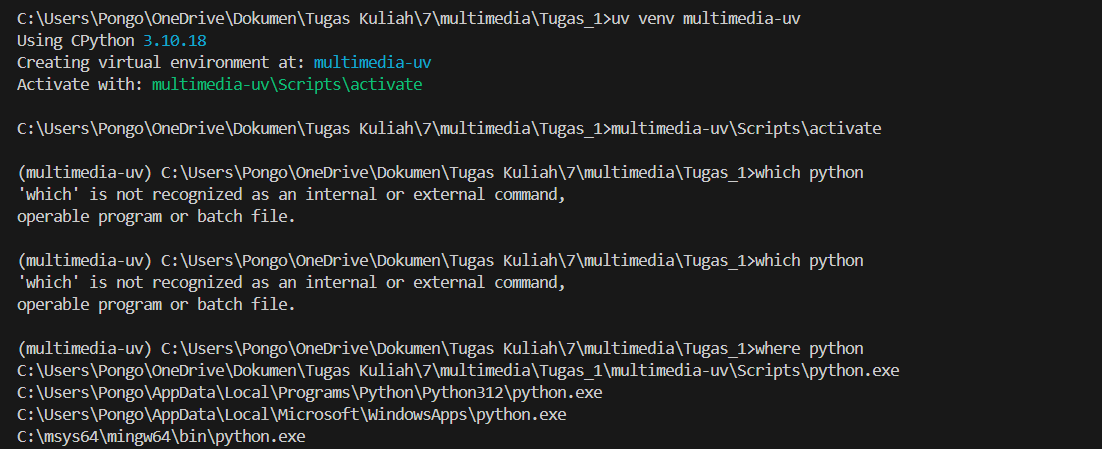
\includegraphics[width=0.8\textwidth]{Figure/gambar1.png}
    \caption{Output verifikasi environment aktif di terminal}
    \label{fig:output_env}
\end{figure}


\subsection{Bagian 2: Instalasi Library Multimedia}
Setelah environment aktif, install library-library berikut:

\subsubsection{Library Audio Processing}
\begin{lstlisting}[language=bash, caption=Instalasi library audio]
# Untuk conda:
conda install -c conda-forge librosa soundfile scipy

# Untuk pip (venv/uv):
pip install librosa soundfile scipy
\end{lstlisting}

\subsubsection{Library Image Processing}
\begin{lstlisting}[language=bash, caption=Instalasi library image]
# Untuk conda:
conda install -c conda-forge opencv pillow scikit-image matplotlib

# Untuk pip (venv/uv):
pip install opencv-python pillow scikit-image matplotlib
\end{lstlisting}

\subsubsection{Library Video Processing}
\begin{lstlisting}[language=bash, caption=Instalasi library video]
# Untuk conda:
conda install -c conda-forge ffmpeg
pip install moviepy

# Untuk pip (venv/uv):
pip install moviepy
\end{lstlisting}

\subsubsection{Library General Purpose}
\begin{lstlisting}[language=bash, caption=Instalasi library umum]
# Untuk conda:
conda install numpy pandas jupyter

# Untuk pip (venv/uv):
pip install numpy pandas jupyter
\end{lstlisting}

\textbf{Dokumentasikan di sini:}
\begin{itemize}
    \item Perintah instalasi yang Anda gunakan
    \begin{enumerate}
        \item pip install librosa soundfile scipy
        \item pip install opencv-python pillow scikit-image matplotlib
        \item pip install moviepy
        \item pip install numpy pandas jupyter
    \end{enumerate}

    \item Screenshot proses instalasi atau output sukses
    
    \begin{minipage}{\linewidth}
        \centering
        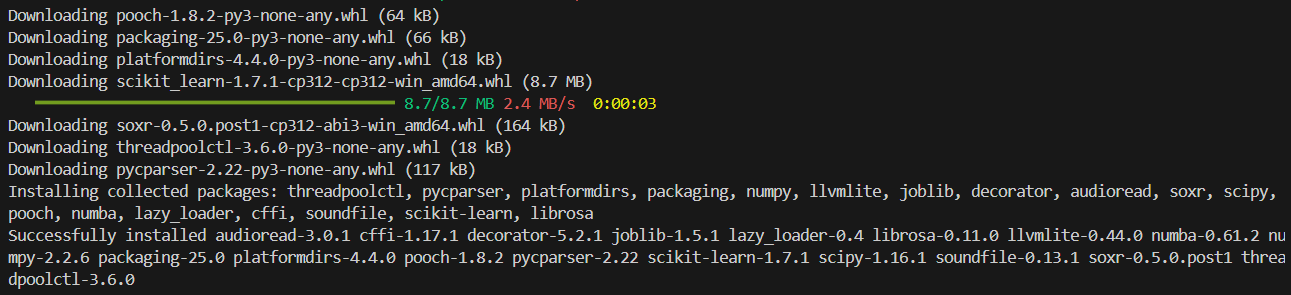
\includegraphics[width=0.8\textwidth]{Figure/output sukses librosa.png}
        \captionof{figure}{Output sukses instalasi librosa, soundfile, scipy di terminal}
        \label{fig:output_librosa}
    \end{minipage}
        
    \begin{minipage}{\linewidth}
        \centering
        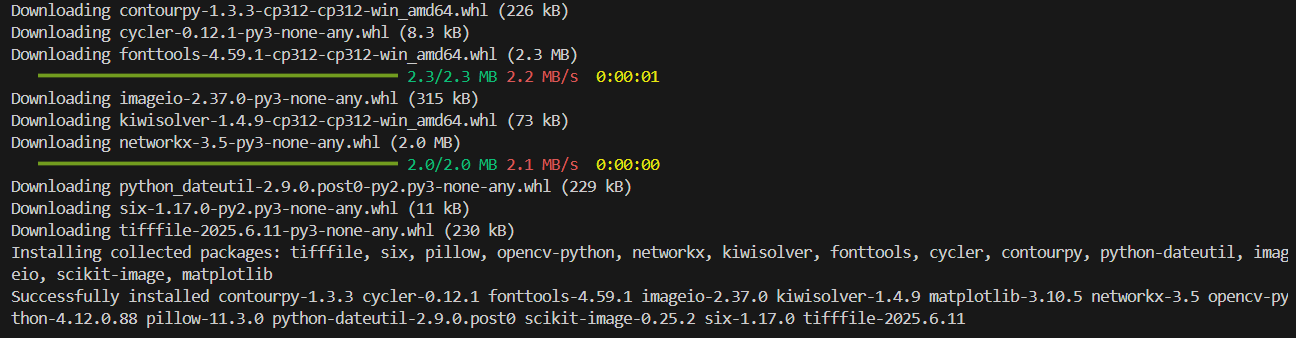
\includegraphics[width=0.8\textwidth]{Figure/output sukses opencv.png}
        \captionof{figure}{Output sukses instalasi opencv, pillow, scikit-image, matplotlib di terminal}
        \label{fig:output_opencv}
    \end{minipage}
        
    \begin{minipage}{\linewidth}
        \centering
        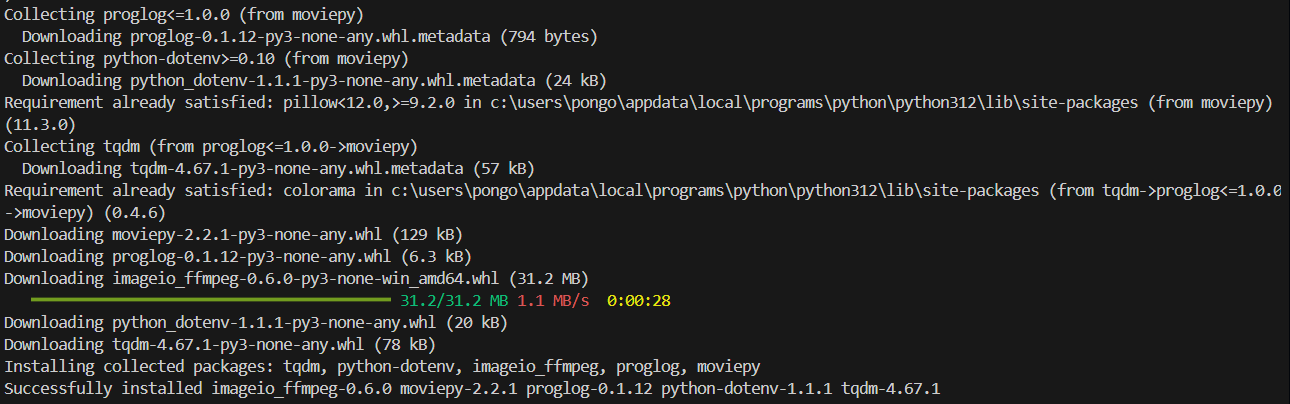
\includegraphics[width=0.8\textwidth]{Figure/output sukses moviepy.png}
        \captionof{figure}{Output sukses instalasi moviepy di terminal}
        \label{fig:output_moviepy}
    \end{minipage}
        
    \begin{minipage}{\linewidth}
        \centering
        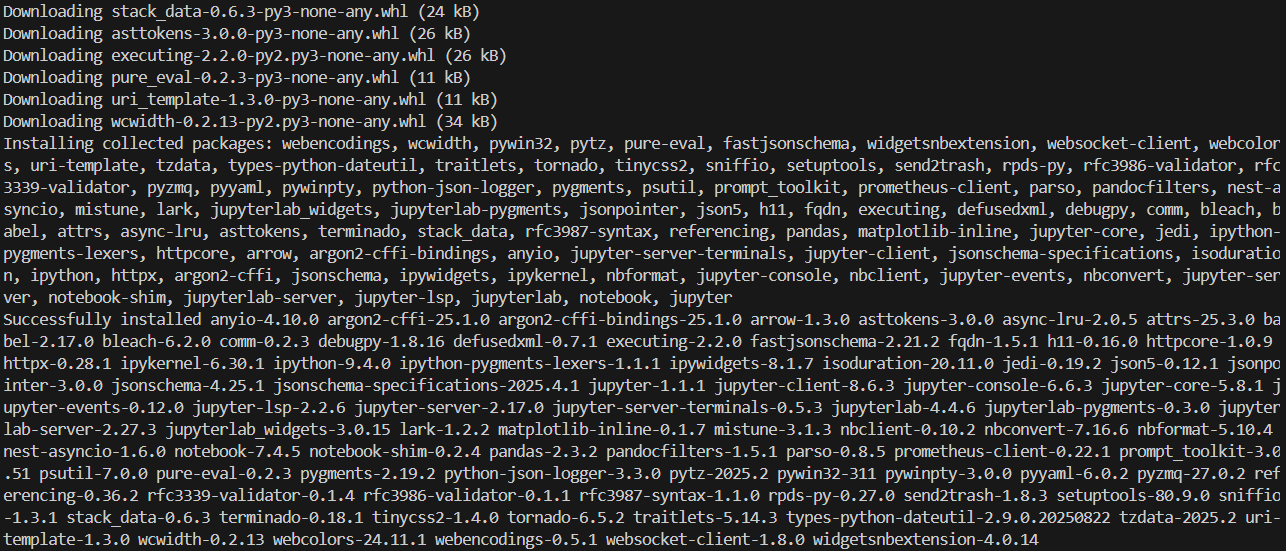
\includegraphics[width=0.8\textwidth]{Figure/output sukses numpy pandas.png}
        \captionof{figure}{Output sukses instalasi numpy, pandas, jupyter di terminal}
        \label{fig:output_numpy}
    \end{minipage}

    \item Daftar library yang berhasil diinstall dengan versinya
    \begin{itemize}
        \item jupyter 1.1.1
        \item librosa 0.11.0
        \item matplotlib 3.10.5
        \item matplotlib-inline 0.1.7
        \item moviepy 2.2.1
        \item numpy 2.2.6
        \item opencv-python 4.12.0.88
        \item pandas 2.3.2
        \item pillow 11.3.0
        \item scikit-image 0.25.2
        \item scipy 1.16.1
        \item soundfile 0.13.1
    \end{itemize}

\end{itemize}


\subsection{Bagian 3: Verifikasi Instalasi}
Buat file Python sederhana untuk menguji semua library yang telah diinstall:


\textbf{Jalankan script dan dokumentasikan hasilnya:}

\begin{lstlisting}[language=Python, caption=Kode script verifikasi instalasi di file test\_multimedia.py]
# Verifikasi-Instalasi.py
print("=== Verifikasi Library ===")

try:
    import librosa
    print(f"librosa sudah terinstal, versi: {librosa.__version__}")
except ImportError:
    print("librosa BELUM terinstal")

try:
    import soundfile
    print(f"soundfile sudah terinstal, versi: {soundfile.__version__}")
except ImportError:
    print("soundfile BELUM terinstal")

try:
    import scipy
    print(f"scipy sudah terinstal, versi: {scipy.__version__}")
except ImportError:
    print("scipy BELUM terinstal")

try:
    import cv2
    print(f"opencv-python sudah terinstal, versi: {cv2.__version__}")
except ImportError:
    print("opencv-python BELUM terinstal")

try:
    import PIL
    print(f"Pillow sudah terinstal, versi: {PIL.__version__}")
except ImportError:
    print("Pillow BELUM terinstal")

try:
    import skimage
    print(f"scikit-image sudah terinstal, versi: {skimage.__version__}")
except ImportError:
    print("scikit-image BELUM terinstal")

try:
    import matplotlib
    print(f"matplotlib sudah terinstal, versi: {matplotlib.__version__}")
except ImportError:
    print("matplotlib BELUM terinstal")

try:
    import moviepy
    print(f"moviepy sudah terinstal, versi: {moviepy.__version__}")
except ImportError:
    print("moviepy BELUM terinstal")

try:
    import numpy
    print(f"numpy sudah terinstal, versi: {numpy.__version__}")
except ImportError:
    print("numpy BELUM terinstal")

try:
    import pandas
    print(f"pandas sudah terinstal, versi: {pandas.__version__}")
except ImportError:
    print("pandas BELUM terinstal")

try:
    import notebook
    print(f"jupyter-notebook sudah terinstal, versi: {notebook.__version__}")
except ImportError:
    print("jupyter-notebook BELUM terinstal")

print("=== Verifikasi selesai ===")
\end{lstlisting}

\begin{figure}[H]
    \centering
    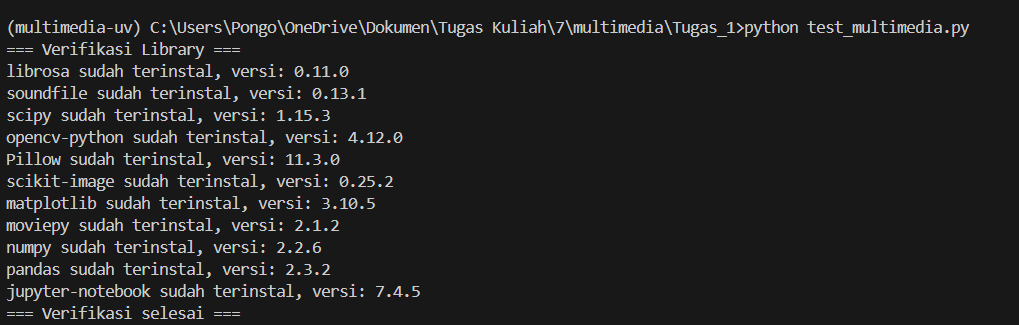
\includegraphics[width=0.9\textwidth]{Figure/test_multimedia.png}
    \caption{Hasil Output dari script test\_multimedia.py}
    \label{fig:output_test_multimedia}
\end{figure}


\subsection{Bagian 4: Simple Test dengan Sample Code}
Buat dan jalankan contoh sederhana untuk setiap kategori multimedia:


\subsubsection{Test Audio Processing}
\begin{lstlisting}[language=Python, caption=Test audio processing sederhana]
import numpy as np
import matplotlib.pyplot as plt

# Generate simple sine wave
duration = 2  # seconds
sample_rate = 44100
frequency = 440  # A4 note

t = np.linspace(0, duration, int(sample_rate * duration))
audio_signal = np.sin(2 * np.pi * frequency * t)

# Plot waveform
plt.figure(figsize=(10, 4))
plt.plot(t[:1000], audio_signal[:1000])  # Plot first 1000 samples
plt.title('Sine Wave (440 Hz)')
plt.xlabel('Time (s)')
plt.ylabel('Amplitude')
plt.grid(True)
plt.savefig('sine_wave_test.png', dpi=150, bbox_inches='tight')
plt.show()

print(f"Generated {duration}s sine wave at {frequency}Hz")
print(f"Sample rate: {sample_rate}Hz")
print(f"Total samples: {len(audio_signal)}")
\end{lstlisting}

\subsubsection{Test Image Processing}
\begin{lstlisting}[language=Python, caption=Test image processing sederhana]
import numpy as np
import matplotlib.pyplot as plt
from PIL import Image

# Create a simple test image
width, height = 400, 300
image = np.zeros((height, width, 3), dtype=np.uint8)

# Add some patterns
image[:, :width//3, 0] = 255  # Red section
image[:, width//3:2*width//3, 1] = 255  # Green section
image[:, 2*width//3:, 2] = 255  # Blue section

# Add a white circle in the center
center_x, center_y = width//2, height//2
radius = 50
Y, X = np.ogrid[:height, :width]
mask = (X - center_x)**2 + (Y - center_y)**2 <= radius**2
image[mask] = [255, 255, 255]

# Display and save
plt.figure(figsize=(8, 6))
plt.imshow(image)
plt.title('Test Image with RGB Stripes and White Circle')
plt.axis('off')
plt.savefig('test_image.png', dpi=150, bbox_inches='tight')
plt.show()

print(f"Created test image: {width}x{height} pixels")
print(f"Image shape: {image.shape}")
print(f"Image dtype: {image.dtype}")
\end{lstlisting}

\textbf{Dokumentasikan hasil eksekusi:}
\begin{itemize}
    \item Screenshot output dari kedua script di atas
    
    \begin{minipage}{\linewidth}
        \centering
        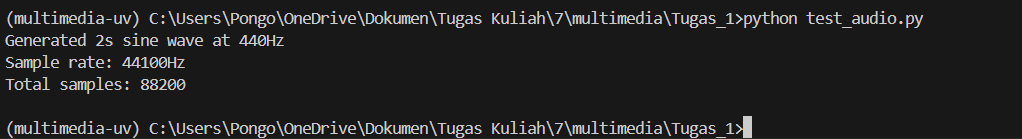
\includegraphics[width=0.8\textwidth]{Figure/output audio.png}
        \captionof{figure}{Output dari script pertama}
        \label{fig:output_script1}
    \end{minipage}

    \begin{minipage}{\linewidth}
        \centering
        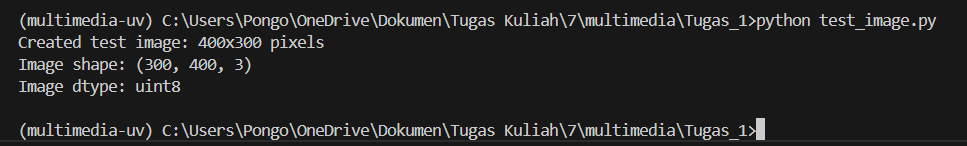
\includegraphics[width=0.8\textwidth]{Figure/output image.png}
        \captionof{figure}{Output dari script kedua}
        \label{fig:output_script2}
    \end{minipage}

    \item Gambar yang dihasilkan (\texttt{sine\_wave\_test.png} dan \texttt{test\_image.png})

    \begin{minipage}{\linewidth}
        \centering
        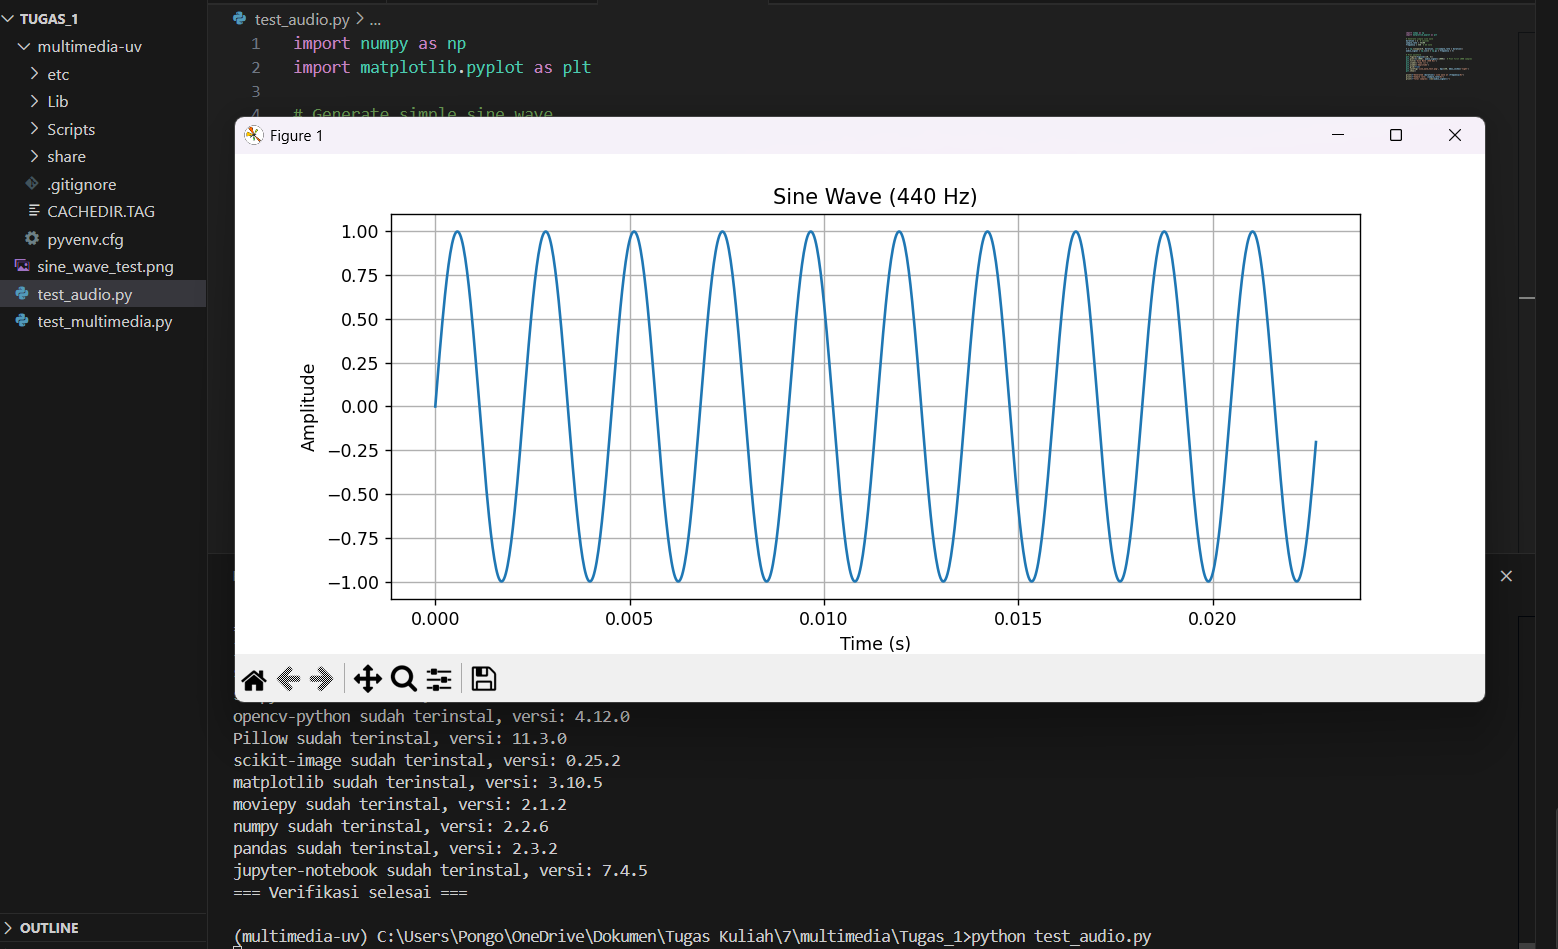
\includegraphics[width=0.6\textwidth]{Figure/gambar audio.png}
        \captionof{figure}{Hasil gambar \texttt{sine\_wave\_test.png}}
        \label{fig:sine_wave}
    \end{minipage}

    \begin{minipage}{\linewidth}
        \centering
        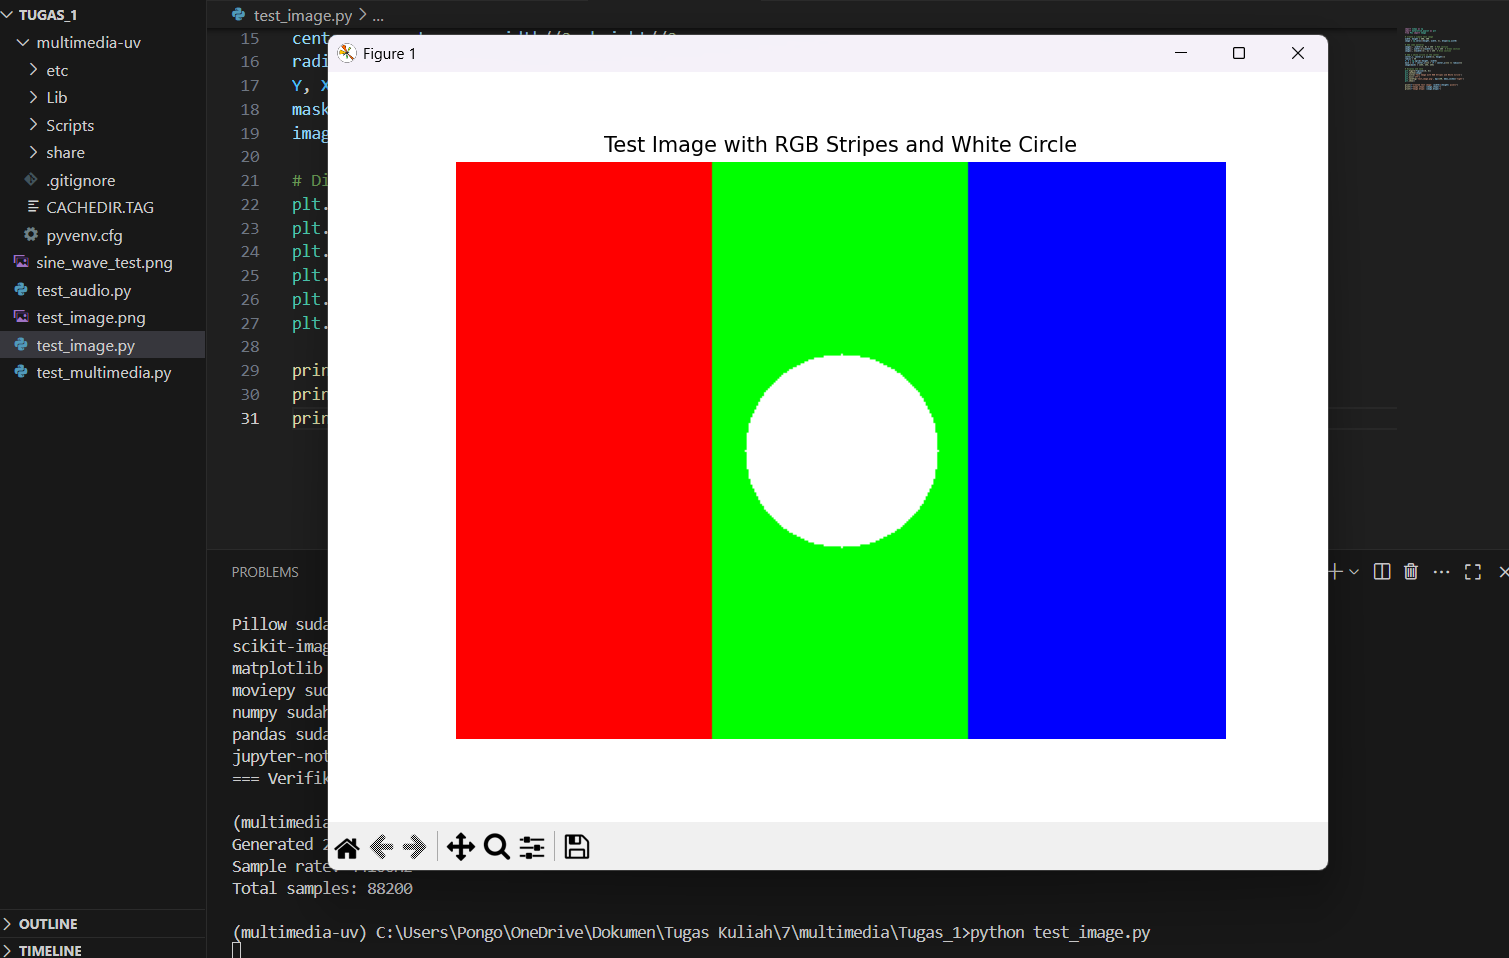
\includegraphics[width=0.6\textwidth]{Figure/gambar image.png}
        \captionof{figure}{Hasil gambar \texttt{test\_image.png}}
        \label{fig:test_image}
    \end{minipage}

    \item Error message jika ada dan cara mengatasinya

\end{itemize}


\section{Bagian Laporan}

\subsection{Output Verifikasi Instalasi}
\textbf{Copy-paste output lengkap dari script \texttt{test\_multimedia.py} di sini:}

\begin{lstlisting}[caption=Output verifikasi instalasi]
    === Verifikasi Library ===
    librosa sudah terinstal, versi: 0.11.0
    soundfile sudah terinstal, versi: 0.13.1
    scipy sudah terinstal, versi: 1.15.3
    opencv-python sudah terinstal, versi: 4.12.0
    Pillow sudah terinstal, versi: 11.3.0
    scikit-image sudah terinstal, versi: 0.25.2
    matplotlib sudah terinstal, versi: 3.10.5
    moviepy sudah terinstal, versi: 2.1.2
    numpy sudah terinstal, versi: 2.2.6
    pandas sudah terinstal, versi: 2.3.2
    jupyter-notebook sudah terinstal, versi: 7.4.5
    === Verifikasi selesai ===
\end{lstlisting}

\subsection{Screenshot Hasil Test}
\textbf{Sisipkan screenshot atau gambar hasil dari:}
\begin{itemize}
    \item Terminal/command prompt yang menunjukkan environment aktif
    
    \begin{minipage}{\linewidth}
        \centering
        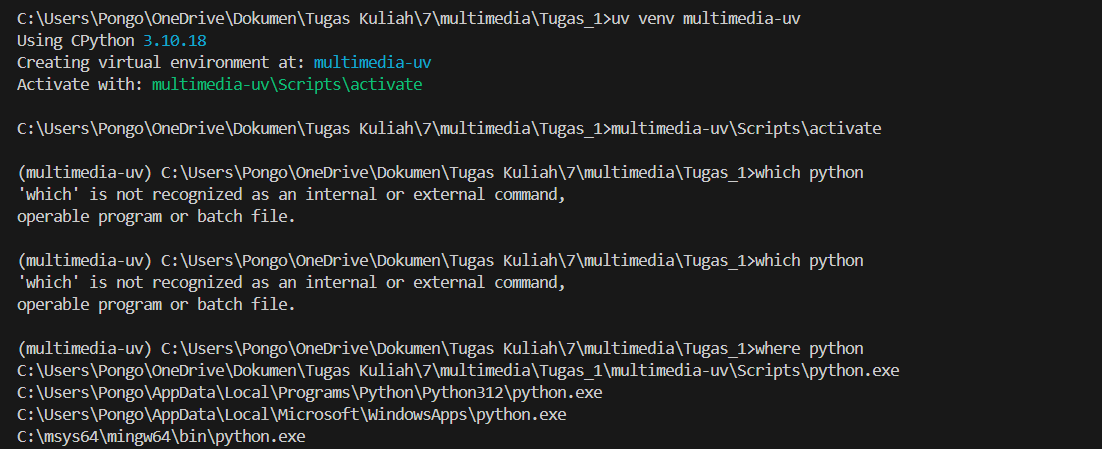
\includegraphics[width=0.8\textwidth]{Figure/gambar1.png}
        \captionof{figure}{Tampilan terminal yang menunjukkan environment aktif}
        \label{fig:env_active}
    \end{minipage}

    \item Output dari script test audio (sine wave plot)
    
    \begin{minipage}{\linewidth}
        \centering
        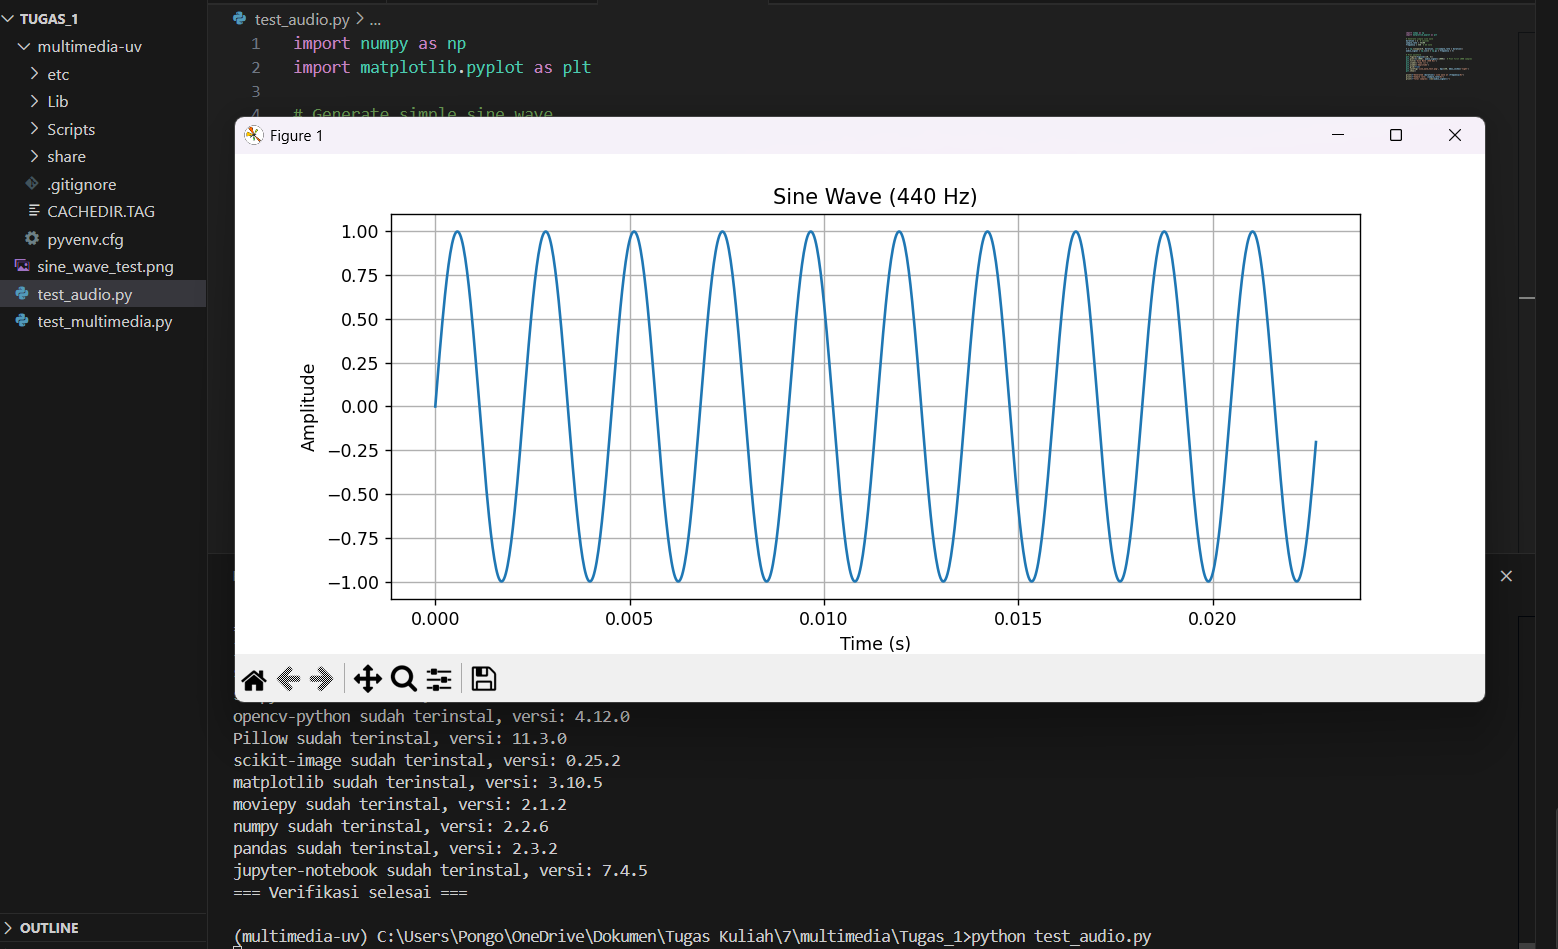
\includegraphics[width=0.8\textwidth]{Figure/gambar audio.png}
        \captionof{figure}{Hasil plot sine wave dari script test audio}
        \label{fig:sine_wave}
    \end{minipage}

    \item Output dari script test image (RGB stripes dengan circle)
    
    \begin{minipage}{\linewidth}
        \centering
        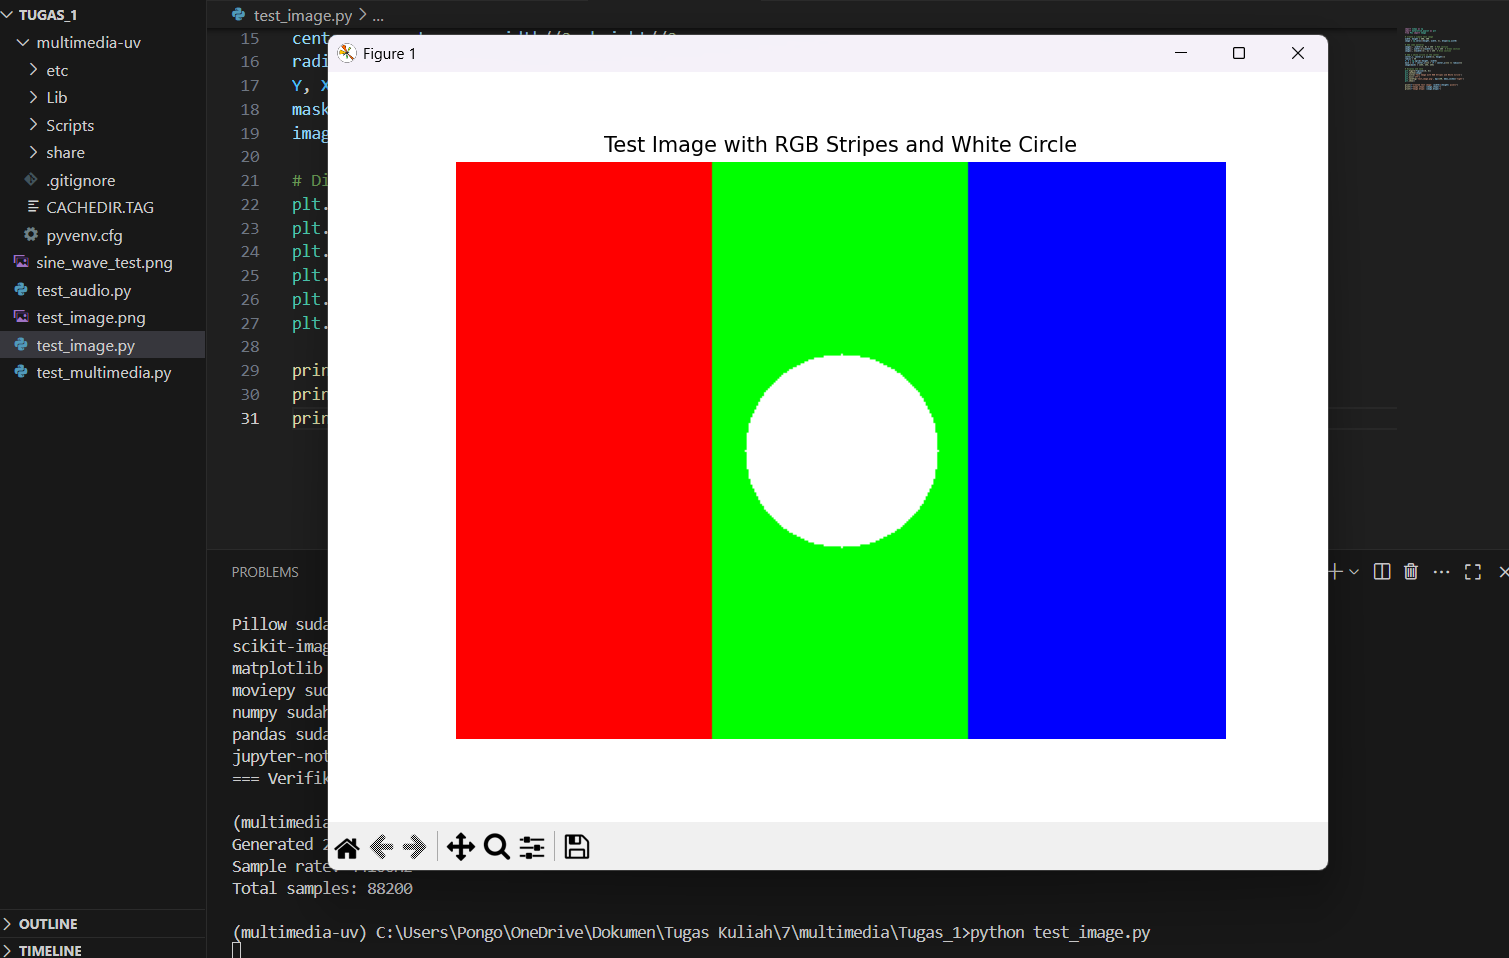
\includegraphics[width=0.8\textwidth]{Figure/gambar image.png}
        \captionof{figure}{Hasil gambar RGB stripes dengan lingkaran dari script test image}
        \label{fig:test_image}
    \end{minipage}
\end{itemize}


\textit{Gunakan perintah \textbackslash\texttt{includegraphics} untuk menyisipkan gambar}

\subsection{Analisis dan Refleksi}
\textbf{Jawab pertanyaan berikut:}

\begin{enumerate}
    \item \textbf{Mengapa penting menggunakan environment terpisah untuk project multimedia?}
    
    \textit{Menurut saya, menggunakan environment terpisan untuk setiap project multimedia itu penting karena setiap project biasanya memiliki kebutuhan library dan versi yang berbeda-beda. Jadi dengan environment terpisah, maka kita dapat menghindari terjadinya konflik antar library yang dapat menyebabkan error.}
    
    \item \textbf{Apa perbedaan utama antara conda, venv, dan uv? Mengapa Anda memilih tool yang Anda gunakan?}
    
    \textit{Berdasarkan informasi yang saya dapatkan di pertemuan pertama kemarin, 
    ketiga tools manajemen environment tersebut memiliki perbedaan utama pada kecepatan, ukuran, serta karakteristik dependency managementnya.}

    \textit{Untuk conda dan venv, memiliki kekurangan dari segi ukuran serta proses instalasinya yang cukup lama. 
    Sedangkan uv memiliki keunggulan dari segi kecepatan dan ukuran yang lebih kecil, meskipun memiliki kekurangan yaitu harus melakukan instalasi ulang setiap berpindah folder project.}

    \item \textbf{Library mana yang paling sulit diinstall dan mengapa?}
    
    \textit{Sebenarnya tidak ada library yang sulit untuk diinstall, hanya saja saya kurang teliti dalam proses instalasi sehingga library terinstall secara global dan bukan di environment aktif yang sebelumnya sudah di buat.}
    
    \item \textbf{Bagaimana cara mengatasi masalah dependency conflict jika terjadi?}
    
    \textit{Melakukan upgrade untuk semua library yang bermasalah, maka uv akan otomatis mengintsall versi yang kompatibel. Kemudian, bisa juga menggunakan uv pip check untuk memeriksa, library mana saja yang bertabrakan versinya, kemudian bisa di hapus ataupun di upgrade.}
    
    \item \textbf{Jelaskan fungsi dari masing-masing library yang berhasil Anda install!}
    \begin{itemize}
        \item \textbf{jupyter:} \textit{Menyediakan notebook interaktif untuk menulis kode, teks, grafik, dan hasil eksekusi}
        \item \textbf{librosa:} \textit{Untuk analisis audio/musik, seperti mengekstrak file audio}
        \item \textbf{matplotlib:} \textit{Untuk membuat grafik, plot, dan chart}
        \item \textbf{moviepy:} \textit{Untuk mengedit dan memproses video}
        \item \textbf{numpy:} \textit{Untuk komputasi numerik dengan array/matriks}
        \item \textbf{opencv-python:} \textit{Library computer vision untuk membaca, memproses, dan menganalisis gambar atau video.}
        \item \textbf{pandas:} \textit{Untuk analisis dan manipulasi data, terutama data berbentuk tabel.}
        \item \textbf{pillow:} \textit{Untuk manipulasi gambar, seperti resize, crop, filter, dan konversi format.}
        \item \textbf{scikit-image:} \textit{Untuk pengolahan citra, termasuk filter dan transformasi gambar.}
        \item \textbf{scipy:} \textit{Menyediakan algoritma untuk optimisasi, aljabar linear, FFT, statistik, dan lain-lain.}
        \item \textbf{soundfile:} \textit{Untuk membaca dan menulis file audio dengan format seperti WAV atau FLAC.}
    \end{itemize}

\end{enumerate}

\subsection{Troubleshooting}
\textbf{Dokumentasikan masalah yang Anda hadapi (jika ada) dan cara mengatasinya:}

\begin{itemize}
    \item \textbf{Masalah 1:} \textit{Kesalahan penggunana which python pada saat verifikasi environment aktif dengan uv.}
    
    \textbf{Solusi:} \textit{Saya mencari informasi melalui chat GPT, dan menemukan bahwa command which python hanya dapat digunakan pada macbook/linux, sedangkan pada windows harus menggunakan command where python.}
    
    \item \textbf{Masalah 2:} \textit{Menginstall library secara global, bukan di environment aktif.}
    
    \textbf{Solusi:} \textit{Saya mencari informasi melalui chat GPT, dan menemukan bahwa saya kurang teliti dalam proses instalasi library. Yang mana ketika saya melakukan instalasi semua library sebelumnya, saya langsung menuliskan command pip install tanpa memastikan bahwa environment yang saya buat sebelumnya sudah aktif. Sehingga semua library yang di install masih berada di global dan bukan berada di environment yang sudah saya buat.}
    \begin{figure}[h!]
        \centering
        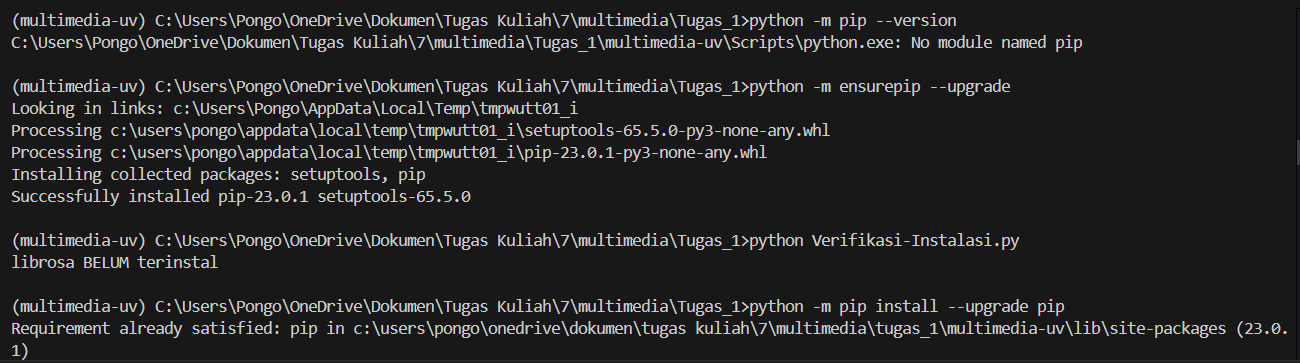
\includegraphics[width=0.9\textwidth]{Figure/solusi.png}
        \caption{Output solusi masalah instalasi library di terminal}
        \label{fig:solusi masalah install library}
    \end{figure}
\end{itemize}

\section{Export Environment untuk Reproduksi}
Sebagai langkah terakhir, export environment Anda agar dapat direproduksi:

\subsection{Untuk Conda}
\begin{lstlisting}[language=bash, caption=Export conda environment]
conda env export > environment.yml
\end{lstlisting}

\subsection{Untuk venv/uv}
\begin{lstlisting}[language=bash, caption=Export pip requirements]
pip freeze > requirements.txt
\end{lstlisting}

\textbf{Copy-paste isi file environment.yml atau requirements.txt di sini:}

\begin{lstlisting}[caption=Environment/Requirements file]
    anyio==4.10.0
    argon2-cffi==25.1.0
    argon2-cffi-bindings==25.1.0
    arrow==1.3.0
    asttokens==3.0.0
    async-lru==2.0.5
    attrs==25.3.0
    audioread==3.0.1
    babel==2.17.0
    beautifulsoup4==4.13.5
    bleach==6.2.0
    certifi==2025.8.3
    cffi==1.17.1
    charset-normalizer==3.4.3
    colorama==0.4.6
    comm==0.2.3
    contourpy==1.3.2
    cycler==0.12.1
    debugpy==1.8.16
    decorator==5.2.1
    defusedxml==0.7.1
    exceptiongroup==1.3.0
    executing==2.2.0
    fastjsonschema==2.21.2
    fonttools==4.59.1
    fqdn==1.5.1
    h11==0.16.0
    httpcore==1.0.9
    httpx==0.28.1
    idna==3.10
    imageio==2.37.0
    imageio-ffmpeg==0.6.0
    ipykernel==6.30.1
    ipython==8.37.0
    ipywidgets==8.1.7
    isoduration==20.11.0
    jedi==0.19.2
    Jinja2==3.1.6
    joblib==1.5.2
    json5==0.12.1
    jsonpointer==3.0.0
    jsonschema==4.25.1
    jsonschema-specifications==2025.4.1
    jupyter==1.1.1
    jupyter-console==6.6.3
    jupyter-events==0.12.0
    jupyter-lsp==2.2.6
    jupyter_client==8.6.3
    jupyter_core==5.8.1
    jupyter_server==2.17.0
    jupyter_server_terminals==0.5.3
    jupyterlab==4.4.6
    jupyterlab_pygments==0.3.0
    jupyterlab_server==2.27.3
    jupyterlab_widgets==3.0.15
    kiwisolver==1.4.9
    lark==1.2.2
    lazy_loader==0.4
    librosa==0.11.0
    llvmlite==0.44.0
    MarkupSafe==3.0.2
    matplotlib==3.10.5
    matplotlib-inline==0.1.7
    mistune==3.1.3
    moviepy==2.2.1
    msgpack==1.1.1
    nbclient==0.10.2
    nbconvert==7.16.6
    nbformat==5.10.4
    nest-asyncio==1.6.0
    networkx==3.4.2
    notebook==7.4.5
    notebook_shim==0.2.4
    numba==0.61.2
    numpy==2.2.6
    opencv-python==4.12.0.88
    overrides==7.7.0
    packaging==25.0
    pandas==2.3.2
    pandocfilters==1.5.1
    parso==0.8.5
    pillow==11.3.0
    platformdirs==4.4.0
    pooch==1.8.2
    proglog==0.1.12
    prometheus_client==0.22.1
    prompt_toolkit==3.0.51
    psutil==7.0.0
    pure_eval==0.2.3
    pycparser==2.22
    Pygments==2.19.2
    pyparsing==3.2.3
    python-dateutil==2.9.0.post0
    python-dotenv==1.1.1
    python-json-logger==3.3.0
    pytz==2025.2
    pywin32==311
    pywinpty==3.0.0
    PyYAML==6.0.2
    pyzmq==27.0.2
    referencing==0.36.2
    requests==2.32.5
    rfc3339-validator==0.1.4
    rfc3986-validator==0.1.1
    rfc3987-syntax==1.1.0
    rpds-py==0.27.1
    scikit-image==0.25.2
    scikit-learn==1.7.1
    scipy==1.15.3
    Send2Trash==1.8.3
    six==1.17.0
    sniffio==1.3.1
    soundfile==0.13.1
    soupsieve==2.7
    soxr==0.5.0.post1
    stack-data==0.6.3
    terminado==0.18.1
    threadpoolctl==3.6.0
    tifffile==2025.5.10
    tinycss2==1.4.0
    tomli==2.2.1
    tornado==6.5.2
    tqdm==4.67.1
    traitlets==5.14.3
    types-python-dateutil==2.9.0.20250822
    typing_extensions==4.15.0
    tzdata==2025.2
    uri-template==1.3.0
    urllib3==2.5.0
    wcwidth==0.2.13
    webcolors==24.11.1
    webencodings==0.5.1
    websocket-client==1.8.0
    widgetsnbextension==4.0.14
\end{lstlisting}

\section{Kesimpulan}
\textbf{Tuliskan kesimpulan Anda mengenai:}
\begin{itemize}
    \item Pengalaman setup Python environment untuk multimedia
    \item Persiapan untuk project multimedia selanjutnya
    \item Saran untuk mahasiswa lain yang akan melakukan setup serupa
\end{itemize}

\textit{Pengalaman yang saya dapatkan selama proses setup python environment ini sebenarnya cukup simple, hanya saja saya kurang fokus dan teliti dalam beberapa langkah, sehingga menyebabkan beberapa masalah ketika proses instalasinya.}

\textit{Untuk persiapan project selanjutnya, mungkin saya harus lebih berkonsentrasi ketika mengikuti step by step nya.}

\textit{Saran dari saya yaitu, untuk dapat lebih cepat dikerjakan, karena menurut saya tugas ini tidak sesimple keliahatannya}

\section{Referensi}
Sertakan referensi yang Anda gunakan selama proses setup dan troubleshooting.

\begin{thebibliography}{9}
    \bibitem{chatgpt}
    OpenAI. \textit{ChatGPT - Conversational AI}. 
    Tersedia di: \url{https://chatgpt.com/share/68b03039-5e04-8006-96cd-cf3ad0606c09} (diakses 28 Agustus 2025).
\end{thebibliography}


\newpage
\bibliographystyle{IEEEtran}
\bibliography{Referensi}
\end{document}